\documentclass{standalone}
\usepackage{tikz}
\usetikzlibrary{fit}

\tikzset{
  pt/.style={circle,minimum size=3pt,fill=#1,inner sep=0},
  red pt/.style={pt=red},
  green pt/.style={pt=green},
  every picture/.style={line width=1pt,inner sep=0pt},
}
\begin{document}
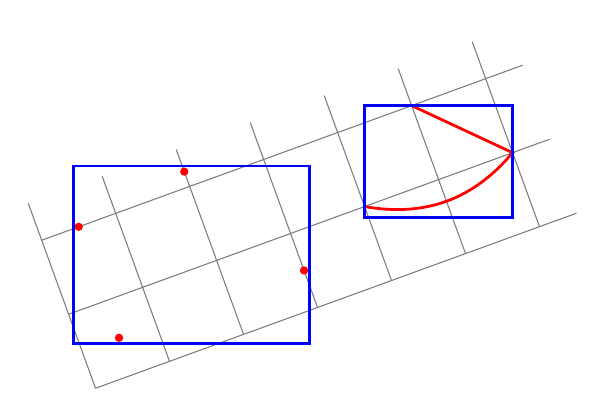
\begin{tikzpicture}[rotate=20]
  \draw[gray,line width=.4pt] (0,0) grid (6.5,2.5);
  % first case: fitting some nodes
  \node[red pt] (a) at (.5,.5){};
  \node[red pt] (b) at (.5,2){};
  \node[red pt] (c) at (3,.5){};
  \node[red pt] (d) at (2,2.2){};
  \begin{scope}[transform shape]
    \node[fit=(a)(b)(c)(d),draw=blue]{};
  \end{scope}
\pgfgettransform{\currtrafo}     %Save the current trafo 

  % second case: fitting arbitrary path
\begin{scope}[local bounding box=bb]
\pgftransformresetnontranslations % Now there is no rotation and it doesn't know 
                                  % things are going to be rotated
\begin{scope}                     % We open a new scope and restore the outer trafo
\pgfsettransform{\currtrafo}      % inside the scope

\draw[red] (4,1) to[bend right] (6,1) -- (5,2);  % Draw anything
\end{scope}                                      % Now the trafo is reset again

\node[fit=(bb),draw=blue]{};     % Externally it doesn't know the content is
                                 % rotated or not

  \end{scope}                    % Back to original trafo.
\end{tikzpicture}
\end{document}
